\chapter{Algorithmen}

Dieses Kapitel beschäftigt sich mit verschiedenen Ansätzen, um den 
Graphabstand zu ermitteln. Im ersten Abschnitt wird versucht, einen 
gemeinsamen induzierten Teilgraphen zu finden. Es wird dabei nicht 
in den ursprünglichen Graphen gesucht sondern in deren Kantengraphen. 
Der zweite Abschnitt beschäftigt sich mit der direkten Suche nach 
einem ECGM in den ursprünglichen Graphen. Dies entspricht der Suche 
nach dem größten gemeinsamen Teilgraph, der jedoch nicht induziert 
sein muss. Algorithmen, die direkt nach einem Graphabstand suchen, 
werden im dritten Abschnitt vorgestellt. 

\section{Algorithmen für MCS}

Die Algorithmen in diesen Abschnitt suchen nach einem MCS. Dabei 
wird nicht der MCS der Originalgraphen ermittelt, sondern der 
Kantengraphen. Dies wird gemacht, weil der MCS ein induzierter 
Teilgraph ist und es passieren kann, dass Knoten ungewollt als 
fehlerhaft oder fehlend angesehen werden (siehe Abschnitt \ref{sec:MCS_Graphabstand}). 

\subsection{McGregor-Algorithmus}\label{sec:McGregor}
Der McGregor-Algorithmus ist ein einfacher Backtracking-Algorithmus. 
Er wurde 1982 erstmalig veröffentlicht und liefert eine exakte 
Lösung. Er wurde unter anderem auch in \cite{MaxCGAlgComp} 
betrachtet. 

\subsubsection{Arbeitsweise}
\begin{lstlisting}[float=htb, caption={McGregor-Algorithmus},label={lst:McGregor}]
Procedure McGregor($comSubgraph$)
    For Each $(u,v) \in V_1 \times V_2$
        If $comSubgraph$.IsAddablePair($u$,$v$) Then

            $comSubgraph$.AddPair($u$,$v$)
        
            If $comSubgraph$.PairCount $>$ $max$.PairCount Then
                $max$ = $comSubgraph$.Clone()
            End If
            
            // Gibt es in beiden Eingabegraphen Knoten, die nicht zum Teilgraphen gehören?
            If $comSubgraph$.IsExpandable Then
                McGregor($comSubgraph$)
            End If
            
            // Backtracking
            $comSubgraph$.RemovePair($u$,$v$)
        End If
    End For
End Procedure
\end{lstlisting}

Das Backtracking wird mittels Rekursion realisiert. Bei jedem 
Rekursionsaufruf ist bereits ein gemeinsamer Teilgraph vorhanden, 
wobei es sich dabei am Anfang um einen leeren Graphen handelt.

Nun werden von den noch möglichen Knotenpaaren der beiden 
Ursprungsgraphen alle durchprobiert. Dabei wird überprüft, ob es 
sich weiterhin um einen induzierten Teilgraphen handelt, wenn das 
aktuelle Knotenpaar zum bisher ermittelten Teilgrpahen hinzugefügt 
wird. Dies ist dann der Fall, wenn zwischen jedem bisherigen 
Knotenpaar $(u_i,v_i)$ sowie dem aktuellen Paar $(u,v)$ entweder in 
beiden Eingabegraphen eine Kante ist, oder in keinem der Graphen 
eine Kante ist ($(u_i,u) \in E_1 \Leftrightarrow (v_i,v) \in E_2$). 
Außerdem darf keiner der Knoten bereits für ein Knotenpaar des 
aktuellen Teilgraphen benutzt worden sein.

Erfüllt ein Knotenpaar diese Bedingungen (is addable), dann wird es zum 
aktuellen Teilgrpahen hinzugefügt. Ist der Teilgraph nun größer als der bisher 
größte, wird er gespeichert. Als nächstes wird überprüft, ob der Teilgraph 
weiterhin vergrößert werden kann. Dies ist dann der Fall, wenn es 
in beiden Eingabegraphen noch Knoten gibt, die nicht zum gemeinsamen Teilgraph 
gehören. Lässt sich der Teilgraph vergrößern (is expandable), dann erfolgt 
ein rekursiver Aufruf, wobei der aktuelle Teilgraph übergeben wird. 
Abschließend wird das aktuelle Paar wieder vom Teilgraphen entfernt, damit 
das nächste Paar überprüft werden kann.

\subsubsection{Beispiel}
Gegeben seien die Graphen in Abbildung \ref{pic:bsp_McGregor_graphs}. Für sie soll nun 
der MCS mittels McGregor-Algorithmus entwickelt werden.

%\begin{figure}[htb]
%\centering
%\hspace*{\fill}
%\subfloat[Der Graph $G_1$]{\includegraphics[width=0.3\linewidth,
%keepaspectratio]{bilder/bsp_McGregor_g1}}
%\hspace*{\fill}
%\subfloat[Der Graph $G_2$]{\includegraphics[width=0.3\linewidth,
%keepaspectratio]{bilder/bsp_McGregor_g2}}
%\hspace*{\fill}
%\caption{Die Graphen $G_1$ und $G_2$}
%\label{pic:bsp_McGregor_graphs}
%\end{figure}

\begin{figure}[htb]
\centering
\hspace*{\fill}
\subfloat[Der Graph $G_1$]{\begin{tikzpicture}
  [normalN/.style={circle,draw,minimum size=0.8cm,thick},
   node distance=1.3cm]

  \node[normalN] (a) {1};
    
  \node[normalN] (b) [right=of a] {2}
    edge [thick] (a);
    
  \node[normalN] (d) [below=of a] {3}
    edge [thick] (a);
  
\end{tikzpicture}}
\hspace*{\fill}
\subfloat[Der Graph $G_2$]{\begin{tikzpicture}
  [normalN/.style={circle,draw,minimum size=0.8cm,thick},
   node distance=1.3cm]

  \node[normalN] (a) {a};
    
  \node[normalN] (b) [right=of a] {b}
    edge [thick] (a);
    
  \node[normalN] (c) [below=of b] {c}
    edge [thick] (b)
    edge [thick] (a);
    
  \node[normalN] (d) [left=of c] {d}
    edge [thick] (a)
    edge [thick] (c);
  
\end{tikzpicture}}
\hspace*{\fill}
\caption{Die Graphen $G_1$ und $G_2$}
\label{pic:bsp_McGregor_graphs}
\end{figure}


Es folgt nun die Betrachtung eines einzelnen Aufrufs der McGregor-Prozedur, 
wobei schon ein Teilgraph ($comSubgraph$) vorgegeben ist. Dabei stellen \emph{rote} Linien 
Kanten in $G_1$ dar und \emph{grüne} Linien Kanten in $G_2$. Ist eine Linie 
gestrichelt, dann bedeutet dies, dass zwischen beiden Knoten keine Kante 
vorhanden ist.

Die Paare $(1,a)$ und $(2,b)$ sind bereits als Teilgraph vorgegeben. 
Als mögliche Paare aus $V_1$ und $V_2$, deren Knoten noch nicht 
verwendet wurden, bleiben noch $(3,c)$ und $(3,d)$. 
Abbildung \ref{pic:bsp_McGregor_pairs} stellt die Überprüfung dar.

%\begin{figure}[htb]
%\centering
%\hspace*{\fill}
%\subfloat[]{\includegraphics[width=0.3\linewidth,
%keepaspectratio]{bilder/bsp_McGregor_3c}}
%\hspace*{\fill}
%\subfloat[]{\includegraphics[width=0.3\linewidth,
%keepaspectratio]{bilder/bsp_McGregor_3d}}
%\hspace*{\fill}
%\caption{Überprüfung von Paaren}
%\label{pic:bsp_McGregor_pairs}
%\end{figure}

\begin{figure}[htb]
\centering
\hspace*{\fill}
\subfloat[]{\begin{tikzpicture}
  [normalN/.style={circle,draw,minimum size=0.8cm,thick},
   node distance=1.3cm]

  \path (0,0)     node[normalN] (l) {1a}
       +(-60:2.1) node[normalN] (b) {3c};
       
  \node[normalN] (r) [right=of l] {2b};

    
  \draw [thick] (l) -- (r);
  
  \draw [thick,red] (l) -- (b);
  \draw [thick,darkgreen,out=-90,in=180] (l) to (b);

  \draw [thick,red,dashed] (r) -- (b);
  \draw [thick,darkgreen,out=-90,in=0] (r) to (b);
    
\end{tikzpicture}}
\hspace*{\fill}
\subfloat[]{\begin{tikzpicture}
  [normalN/.style={circle,draw,minimum size=0.8cm,thick},
   node distance=1.3cm]

  \path (0,0)     node[normalN] (l) {1a}
       +(-60:2.1) node[normalN] (b) {3d};
       
  \node[normalN] (r) [right=of l] {2b};

    
  \draw [thick] (l) -- (r);
  
  \draw [thick,red] (l) -- (b);
  \draw [thick,darkgreen,out=-90,in=180] (l) to (b);

  \draw [thick,red,dashed] (r) -- (b);
  \draw [thick,dashed,darkgreen,out=-90,in=0] (r) to (b);
    
\end{tikzpicture}}
\hspace*{\fill}
\caption{Überprüfung von Paaren}
\label{pic:bsp_McGregor_pairs}
\end{figure}

Das Paar $(3,c)$ wird 
zuerst überprüft. Es kann jedoch nicht zum gemeinsamen Teilgraphen hinzugefügt 
werden, weil es eine Kante $(b,c)$ in $G_2$ gibt, jedoch keine 
Kante $(2,3)$ in $G_1$.

Als nächstes überprüft der Algorithmus das Paar $(3,d)$. Die Kanten $(1,3)$ 
und $(a,d)$ sind in $G_1$ und $G_2$ vorhanden. Außerdem sind weder $(2,3)$ 
noch $(b,d)$ in $G_1$ bzw. $G_2$ vorhanden. Somit kann $(3,d)$ zum 
Teilgraphen hinzugefügt werden. 

Nach dem Hinzufügen des Paars zum Teilgraphen, wird der neue gemeinsame 
Teilgraph mit dem bisherigen größten verglichen und gegebenenfalls gespeichert. 
Im nächsten Schritt wird überprüft, ob der Teilgraph erweitert werden kann. 
Dies ist nicht der Fall, da bereits alle Knoten aus $G_1$ verbraucht wurden. 
Zuletzt wird das Paar $(3,d)$ wieder entfernt, um andere Möglichkeiten zu probieren 
(die es in diesem Beispiel jedoch nicht gibt). 

\subsection{MIS-basierter Algorithmus}
Der folgende Algorithmus basiert auf einem Verfahren, das in \cite{MaxCSwitMaxIS} 
vorgestellt wurde. Er arbeitet mit dem Assoziationsgraphen der zu 
vergleichenden Graphen und sucht dort ein MIS (siehe Abschnitt \ref{sec:MIS_MCS}). 


\subsubsection{Arbeitweise}
\begin{lstlisting}[float=htbp,caption={MIS-basierter Algorithmus},label={lst:MIS}]
Procedure MaxIndSet($G_1$,$G_2$)

    $(V_A,E_A)$ = AssoziationsGraph($G_1$,$G_2$)
    $max$ = $\emptyset$ 
    
    // aktuelles independent set
    $selectedNodes$ = $\emptyset$
    
    // Menge der blockierten Knoten
    $blockedNodes_0$ = $\emptyset$
    
    MIS($1$)
    
End Procedure

Procedure MIS($i$)

    // Blockierung übernehmen.
    $blockedNodes_i$ = $blockedNodes_{i-1}$.Clone()
    
    // Alle unblockierten Knoten testen.
    For Each $v \in V_A \backslash blockedNodes_i$
    
        $selectedNodes$ = $selectedNodes \cup \{v\}$
        $blockedNodes_i$ = $blockedNodes_i \cup \{v\}$
    
        // Jeden Nachbarknoten von $v$ blockieren.
        For Each $(v,u) \in E_A$
            $blockedNodes_i$ = $blockedNodes_i \cup \{u\}$
        End For
        
        If $|selectedNodes| > |max|$ Then
            $max$ = $selectedNodes$
        End If
        
        MIS($i+1$)
        
        // Backtracking
        $selectedNodes$ = $selectedNodes \backslash \{v\}$
       
    End For
End Procedure
\end{lstlisting}

Im ersten Schritt baut der Algorithmus den Assoziationsgraphen für die gegebenen 
Graphen auf. Als nächstes wird im Assoziationsgraph nach einem independent set 
gesucht. Dies erfolgt über rekursiv implementiertes Backtracking. Bei jedem 
Rekursionsaufruf ist bereits ein Menge an gewählten Knoten ($selectedNodes$), 
die ein independent set darstellen, vorhanden, wobei es sich 
dabei am Anfang um eine leere Menge handelt.

Bei jedem Rekursionsaufruf wird nun nacheinander jeder Knoten $v$, der nicht zur 
Menge der blockierten Knoten ($blockedNodes$) gehört, zur aktuellen Knotenmenge 
hinzugefügt. Anschließend wird $v$ ebenfalls blockiert.

Ein Knoten wird immer dann 
blockiert, wenn er bereits zum aktuellen independent set gehört oder er nicht 
zur aktuellen Knotenmenge hinzugefügt werden kann, weil sie dann kein inependent 
set mehr ist.

Da ein independent set sich dadurch definiert, dass es keine Kanten 
besitzt, schließt die Wahl von $v$ auch alle Knoten $u$ aus, die über eine Kante 
mit $v$ verbunden sind. Auch sie werden blockiert.

Nun erfolgt der rekursive Aufruf. Abschließend wird $v$ wieder aus 
dem aktuellen independent set entfernt. Auch die Blockierungen der 
Knoten müssen wieder aufgehoben werden. In der in Listing~\ref{lst:MIS} 
dargestellten Umsetzung ist dies dadurch gelöst, dass es für jede 
Rekursionstiefe eine separate Menge von blockierten Knoten gibt. Diese 
lassen sich jeweils über einen Index ansprechen.

\subsubsection{Anpassung an einen Kantengraph}
Handelt es sich bei den gegebenen Graphen um Kantengraphen, so lässt 
sich der Assoziationsgraph $A$ vereinfachen. Jeder Knoten in $A$ 
 steht dann für eine Zuordnung eines Knotens von 
$k(G_1)$ zu einem Knoten aus $k(G_2)$. Es ist jedoch nicht möglich, 
zwei Knoten einander zuzuordnen, wenn einer der Knoten einen Knoten 
in $G_1$ darstellt und der andere eine Kante in $G_2$. Sämtliche Knoten, die 
eine solche Zuordnung darstellen, können somit aus dem Assoziationsgraph 
entfernt werden.

\subsection{Weitere Verfahren}
Es existieren noch weitere Verfahren, um einen MCS zweier Graphen zu ermitteln. 
Aufgrund der verwendeten Eigenschaften, ist jedoch vermutlich keine bessere 
Laufzeit zu erwarten.

In \cite{MCSviaVertexCover} wird ein Verfahren vorgestellt, welches mit 
dem Vertex Cover einer der Graphen arbeitet. Ein Vertex Cover eines Graphen ist 
eine Knotenmenge, bei der jede Kante des Graphen an mindestens einem 
Ende mit einem der Knoten verbunden ist. Ist ein Vertex Cover gefunden, 
wird anschließend mit dem Vertex Cover statt dem gesamten Gaphen 
weitergearbeitet. Insgesamt wird 
das ursprüngliche Problem auf drei kleinere Probleme 
aufgeteilt. Dies ist vermutlich\footnote{\cite{MCSviaVertexCover} geht nicht ausreichend 
darauf ein.} der Grund für die deutlich geringe Laufzeit gegenüber oben genannten 
Verfahren. 

Dass dieses Verfahren bei einem Kantengraph den gleichen Unterschied in der Laufzeit 
zeigt, ist nicht zu erwarten. Das minimale Vertex Cover eines Kantengraphs entspricht 
der Menge der Knoten des ursprünglichen Graphen\footnote{Dies gilt, falls der Graph 
mehr Kanten als Knoten besitzt und zusammenhängend ist. Besitzt der Graph mehr Knoten 
als Kanten, so ergibt sich das minimale Vertex Cover für den Kantengraph aus der Menge 
der Kanten. Bei nicht zusammenhängenden Graphen kann jeder zusammenhängende Teilgraph 
separat betrachtet werden.}. Die Folge ist, dass das Problem nicht aufgeteilt wird. 
Es bleibt in seiner ursprünglichen Größe vorhanden. 

\section{Direkte Suche nach einem ECGM}
Betrachtet man einen Kantengraph statt einem normalen, so bringt dies Vorteile. 
Zum einen lässt sich aus dem MCS der Kantengraphen auch ein ECGM der ursprünglichen 
Graphen ableiten. Zum anderen bietet sich die Möglichkeit, gemeinsame freie 
Kanten zu erhalten, auch wenn die dazugehörigen Knoten nicht Teil eines gemeinsamen 
Teilgraphen sind.

Angenommen, eine solche freie Kante enthält keine zusätzlichen nutzbringenden 
Informationen. In einem solchen Fall kann man direkt nach einem ECGM suchen. Die 
Algorithmen in diesem Abschnitt ermitteln ein solches ECGM. 

\subsection{Vorüberlegungen}\label{Vorueberlegungen}
Der Graphabstand zweier Graphen $G_1=(V_1,E_1)$ und $G_2=(V_2,E_2)$ ergibt sich aus 
den Kosten für das Entfernen und Hinzufügen ungleicher Elemente. Folglich ist der 
Graphabstand minimal, wenn die Menge gemeinsamer Elemente möglichst groß ist. Diese 
Menge wird durch das ECGM $\varphi:\hat{V}_1 \rightarrow \hat{V}_2$ dargestellt. 
Dabei gelte $|V_1| \leq |V_2|$. 

\begin{myTheo}\label{alleVausV1enthalten}
Gegeben seien zwei Graphen $G_1=(V_1,E_1)$ und $G_2=(V_2,E_2)$ mit 
$|V_1|\leq|V_2|$, ein ECGM $\varphi:\hat{V}_1 \rightarrow 
\hat{V}_2$ und dessen Kostenfunktion $c(\varphi)$ mit $c_{nd}(u) + c_{na}(v) > 0$ 
für alle $(u,v) \in V_1 \times V_2$. Ist $c(\varphi)$ minimal, dann ist $\hat{V}_1=V_1$.
\end{myTheo}

\begin{myProof}
Angenommen, $c(\varphi)$ sei minimal, jedoch sei $\hat{V}_1\subset V_1$. Dann
existiert ein Knoten $u \in V_1 \backslash \hat{V}_1$, sowie ein Knoten $v\in V_2
\backslash \hat{V}_2$.

Es sei nun $\lambda:\hat{V}_1 \cup \{u\} \rightarrow \hat{V}_2
\cup \{v\}$ ein weiteres ECGM. Dabei gelte:
\[
\lambda(x)=\left\{\begin{array}{ll}v & x = u \\
                                   \varphi(x) & \text{sonst}
                  \end{array}\right.
\]

Die Kosten für $\lambda$ ergeben sich nun aus den Kosten von $\varphi$, 
jedoch entfallen die Kosten für das Hinzufügen und Entfernen der Knoten 
$u$ und $v$.
\[ c(\lambda)=c(\varphi)-(c_{nd}(u)+c_{na}(v)). \]

Da $c_{nd}(u) + c_{na}(v)>0$ ist, gilt somit $c(\lambda)<c(\varphi)$. 
Somit kann $c(\varphi)$ nicht minimal sein. \qed
\end{myProof}

Satz \ref{alleVausV1enthalten} sagt aus, dass in einem ECGM 
mit minimalen Kosten 
alle Knoten des kleineren Graphen $G_1$ vorhanden sind. Ein 
ECGM lässt sich somit als Permutation der Knoten in $V_2$ 
mit der Größe $|V_1|$ darstellen: Steht ein Knoten $v$ aus $V_2$ 
an $i$-ter Position in der Permutation, wird er dem $i$-ten Knoten 
aus $V_1$ zugeordnet. Ist $v$ nicht in der Permutation vorhanden, 
dann wird ihm kein Knoten zugeordnet.

\subsubsection{Bewertung}
Die Bewertung einer Permutation erfolgt über die Kanten. Dazu werden 
die Knotenpaare $(u_1,v_1)$ aus $G_1$ mit den dazugehörigen Paaren 
$(u_2,v_2)=(\varphi(u_1),\varphi(v_1))$ aus $G_2$ verglichen. Befindet sich 
zwischen beiden Paaren eine Kante, dann wird $(u_1,v_1)$ als gleiches 
Paar mit Kante gezählt. Ist weder zwischen $(u_1,v_1)$ noch zwischen 
$(u_2,v_2)$ eine Kante, handelt es sich lediglich um ein gleiches Paar 
ohne Kante. Alle anderen Paare werden als ungleich betrachtet. 

Eine Permutation $P$ gilt als größer als eine Permutation $Q$, wenn die 
Anzahl der gleichen Paare mit Kante in $P$ größer ist als in $Q$. 
Ist die Anzahl in beiden Permutationen gleich, so ist die Anzahl der 
gleichen Paare ohne Kante entscheidend.

\subsubsection{Beispiel}
Als Beispiel seien erneut die Graphen aus Abschnitt \ref{sec:McGregor} 
gegeben (Abbildung \ref{pic:bsp_Permut_graphs}). Da $G_1$ der kleinere 
der beiden Graphen ist, wird eine dreielementige Permutation der Knoten 
aus $G_2$ gesucht. Insgesamt gibt es 24 mögliche Permutationen, von 
denen nun zwei betrachtet werden.

\begin{figure}[htb]
\centering
\hspace*{\fill}
\subfloat[Der Graph $G_1$]{\begin{tikzpicture}
  [normalN/.style={circle,draw,minimum size=0.8cm,thick},
   node distance=1.3cm]

  \node[normalN] (a) {1};
    
  \node[normalN] (b) [right=of a] {2}
    edge [thick] (a);
    
  \node[normalN] (d) [below=of a] {3}
    edge [thick] (a);
  
\end{tikzpicture}}
\hspace*{\fill}
\subfloat[Der Graph $G_2$]{\begin{tikzpicture}
  [normalN/.style={circle,draw,minimum size=0.8cm,thick},
   node distance=1.3cm]

  \node[normalN] (a) {a};
    
  \node[normalN] (b) [right=of a] {b}
    edge [thick] (a);
    
  \node[normalN] (c) [below=of b] {c}
    edge [thick] (b)
    edge [thick] (a);
    
  \node[normalN] (d) [left=of c] {d}
    edge [thick] (a)
    edge [thick] (c);
  
\end{tikzpicture}}\hspace*{\fill}
\caption{Die Graphen $G_1$ und $G_2$}
\label{pic:bsp_Permut_graphs}
\end{figure}

Die Darstellung der Permutationen erfolgt analog zu Abschnitt \ref{sec:McGregor}. 
Paare aus $G_1$ sind \emph{rot}, Paare aus $G_2$ \emph{grün}. Besitzen Paare eine 
Kante, so ist die dazugehörige Linie durchgezogen. Ist keine Kante vorhanden, dann 
ist die Linie gestrichelt.

%\begin{figure}[htb]
%\centering
%\hspace*{\fill}
%\subfloat[Permutation $P_1$\label{pic:bsp_Permut_abd}]
%         {\includegraphics[width=0.3\linewidth,keepaspectratio]{bilder/bsp_Permut_abd}}
%\hspace*{\fill}
%\subfloat[Permutation $P_2$\label{pic:bsp_Permut_dbc}]
%         {\includegraphics[width=0.3\linewidth,keepaspectratio]{bilder/bsp_Permut_dbc}}
%\hspace*{\fill}
%\caption{Überprüfung von Paaren}
%
%\end{figure}

\begin{figure}[htb]
\centering
\hspace*{\fill}
\subfloat[Permutation $P_1$\label{pic:bsp_Permut_abd}]
{\begin{tikzpicture}
  [normalN/.style={circle,draw,minimum size=0.8cm,thick},
   node distance=1.3cm]

  \path (0,0)     node[normalN] (l) {1a}
       +(-60:2.1) node[normalN] (b) {3d};
       
  \node[normalN] (r) [right=of l] {2b};

    
  \draw [thick,red] (l) -- (r);
  \draw [thick,darkgreen,out=45,in=135] (l) to (r);
  
  \draw [thick,red] (l) -- (b);
  \draw [thick,darkgreen,out=-90,in=180] (l) to (b);

  \draw [thick,red,dashed] (r) -- (b);
  \draw [thick,darkgreen,out=-90,in=0,dashed] (r) to (b);
    
\end{tikzpicture}}
\hspace*{\fill}
\subfloat[Permutation $P_2$\label{pic:bsp_Permut_dbc}]
{\begin{tikzpicture}
  [normalN/.style={circle,draw,minimum size=0.8cm,thick},
   node distance=1.3cm]

  \path (0,0)     node[normalN] (l) {1d}
       +(-60:2.1) node[normalN] (b) {3c};
       
  \node[normalN] (r) [right=of l] {2b};

    
  \draw [thick,red] (l) -- (r);
  \draw [thick,darkgreen,out=45,in=135,dashed] (l) to (r);
  
  \draw [thick,red] (l) -- (b);
  \draw [thick,darkgreen,out=-90,in=180] (l) to (b);

  \draw [thick,red,dashed] (r) -- (b);
  \draw [thick,darkgreen,out=-90,in=0] (r) to (b);
    
\end{tikzpicture}}
\hspace*{\fill}
\caption{Überprüfung von Paaren}
\end{figure}


Die Permutation $P_1=(a,b,d)$ ist in Abbildung \ref{pic:bsp_Permut_abd} dargestellt. 
Die Paare $(1,2)$, $(1,3)$, $(a,b)$ und $(a,d)$ besitzen alle eine Kante. Die Paare 
$(2,3)$ und $(b,d)$ haben beide keine Kante. Somit hat $P_1$ zwei gemeinsame Paare 
mit Kanten und ein gemeinsames Paar ohne Kante.

Die Permutation $P_2=(d,b,c)$ ist in Abbildung \ref{pic:bsp_Permut_dbc} dargestellt. 
Die Paare $(1,3)$ und $(a,c)$ besitzen beide eine Kante. Die Paare 
$(1,2)$ und $(d,b)$ sowie $(2,3)$ und $(b,c)$ haben entweder eine Kante in $G_1$ oder 
in $G_2$, jedoch nicht in beiden gleich. Somit hat $P_2$ nur ein gemeinsames Paar 
mit Kante.

\subsection{Probieren aller Permutationen}
Die einfachste Variante, die beste Permutation zu finden, ist es, alle Permutation 
zu probieren. Die Permutationen können iterativ erzeugt werden. Dabei wird eine 
Permutation direkt aus ihrem Vorgänger gebildet, bis die letzte Permutation erreicht 
ist.

\begin{lstlisting}[float=h, caption={Probieren aller Permutationen},label={lst:Permut}]
Procedure Permut($G_1$,$G_2$)
    $P$ = firstPermut($V_1$,$V_2$)
    $P_{max}$ = $P$
    Do Until isLastPermut($P$)
        If $P > P_{max}$ Then
            $P_{max}$ = $P$
        End If
        $P$ = nextPermut($P$,$V_1$,$V_2$)
    End Do
End Procedure
\end{lstlisting}

Eine Alternative zu einer iterativen Erzeugung von Permutationen ist es, alle 
Möglichkeiten rekursiv zu durchsuchen. Dadurch wird ein Suchbaum erzeugt, dessen 
Blätter eine Permutation darstellen. Ein solches Verfahren kann schneller als 
ein iteratives sein, wenn das Erzeugen einer Permutation aus einer bestehenden 
rechenaufwendig wird. Die Komplexität ändert sich jedoch nicht, denn die 
Anzahl der Permutationen (und somit die Anzahl der Blätter im Suchbaum) bleibt gleich. 

\subsection{Ein Branch-and-Bound-Verfahren}\label{BBAlgo}
Bei einem Branch-and-Bound-Verfahren (B\&B) wird ein Suchbaum aufgebaut, dessen 
Blätter eine mögliche Lösung darstellen. Die Suchstrategie innerhalb des Baums 
unterscheidet sich jedoch von einer Tiefen- oder Breitensuche. Das Verfahren wurde 
erstmals 1960 in \cite{BBOrginal} vorgestellt.

\subsubsection{Arbeitsweise}
Jeder Knoten erhält einen Wert, der eine obere bzw. untere (abhängig davon, ob ein 
Maximum oder Minimum gesucht wird) Schranke für alle Lösungen des Teilbaums angibt. 
Das bedeutet, dass keine der Lösungen in dem Teilbaum besser sein kann, als am 
aktuellen Knoten abgeschätzt wird. 
Bei der Wurzel des Baums beginnend wird der Suchbaum schrittweise an dem Knoten 
erweitert, der die beste Lösung verspricht. Ist der Knoten mit dem besten Wert ein 
Blatt, dann stellt er eine optimale Lösung dar. 

\begin{lstlisting}[float=h, caption={Prinzip des Branch-and-Bound-Algorithmus},label={lst:BB}]
Procedure BB()

    $pQ$ = New PriorityQueue()
    $pQ$.Enqueue($rootNode$)

    Do Until isLeaf($pQ$.Top())
        $top$ = $pQ$.Dequeue()

        For Each $node$ In expand($top$)
            $pQ$.Enqueue($node$)
        End For
    End Do
End Procedure
\end{lstlisting}

Der Vorteil eines B\&B-Verfahrens ist, dass nicht der gesamte Baum durchsucht werden 
muss. Aufgrund der Schranken müssen bestimmte Teilbäume nicht durchsucht werden. 
Nachteilig ist allerdings ein erhöhter Speicheraufwand. Jeder Knoten, der im 
nächsten Schritt expandiert werden kann, muss gespeichert werden. 
Ob der Vorteil oder der Nachteil überwiegt, hängt stark von der gewählten Schranke ab. 
Bildet sich eine deutliche Lösung heraus, wird der Baum nur selten erweitert. Somit 
sind Zeit- und Speicheraufwand gering. Sind alle Knoten etwa gleichwertig, muss der 
Baum häufiger erweitert werden. Im ungünstigsten Fall wird der Suchbaum fast komplett 
aufgespannt. Sowohl Zeit- wie Speicheraufwand sind dann sehr hoch. 

\subsubsection{Beispiel}

%\begin{figure}[htb]
%\centering
%\includegraphics[width=0.7\linewidth,keepaspectratio]{bilder/bsp_BnB_1.png}
%\caption{Beispiel-Suchbaum für das B\&B-Verfahren}
%\label{pic:bsp_BnB_1}
%\end{figure}
Als Beispiel sei der Suchbaum in Abbildung \ref{pic:bsp_BnB_1} gegeben. In diesem soll 
das Minimum ermittelt werden. Es wird also das Blatt mit minimalem Wert gesucht. Der Wert 
der Knoten, die keine Blätter sind, gibt an, wie hoch die Werte der entsprechenden Blätter mindestens sind. 
Dieser Wert entspricht also einer unteren Schranke.


\begin{figure}[htb]
\centering
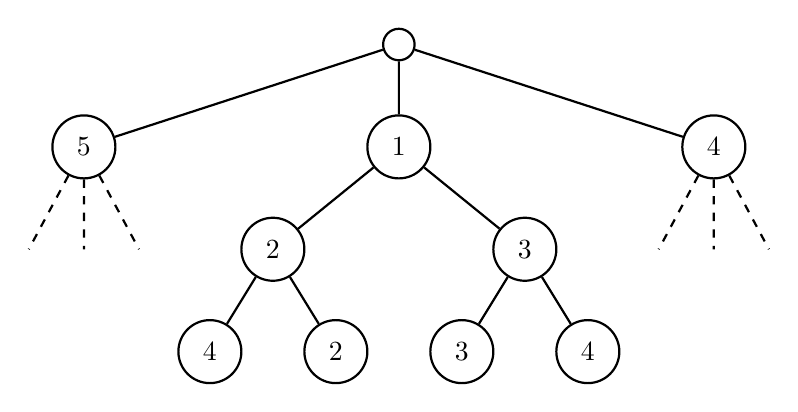
\begin{tikzpicture}
  [normalN/.style={circle,draw,minimum size=0.8cm},
   level 1/.style={sibling distance=4cm},
   level 3/.style={sibling distance=1.6cm},
   level distance=1.3cm,thick,
   node distance=1.3cm]
   

 \node [normalN,minimum size=0.4cm] (root) {}
   child {
     node [normalN] {5} [sibling distance=7mm] child[dashed] child[dashed] child[dashed]
   }
   child {
     node [normalN] {1} [sibling distance=3.2cm]
       child {
         node [normalN] {2}
         child {node [normalN] {4}}
         child {node [normalN] {2}}
       }
       child {
         node [normalN] {3}
         child {node [normalN] {3}}
         child {node [normalN] {4}}
       }
   }
   child {
     node [normalN] {4} [sibling distance=7mm] child[dashed] child[dashed] child[dashed]
   };

\end{tikzpicture}
\caption{Beispiel-Suchbaum für das B\&B-Verfahren}
\label{pic:bsp_BnB_1}
\end{figure}

Abbildung \ref{pic:bsp_BnB} zeigt den Verlauf des Verfahrens für diesen Suchbaum. 
Die Knoten, die zurzeit betrachtet werden, sind \emph{schwarz} dargestellt. 
Der Knoten mit dem minimalen Wert ist zusätzlich \emph{grün} eingefärbt. Knoten, 
die bereits betrachtet wurden und nicht mehr im Speicher sind, sind ausgegraut.

Begonnen wird mit den Unterknoten der Wurzel: $(5)$, $(1)$ und 
$(4)$. Da $(1)$ das Minimum ist, wird an dieser Stelle erweitert. 
Dazu werden die Unterknoten zur Menge der aktuellen Knoten 
hinzugefügt und $(1)$ entfernt.

Im nächsten Schritt wird der Knoten $(2)$ erweitert. Im Speicher 
befinden sich danach die Knoten $(5)$, $(4)$, $(5)$, $(3)$ und 
$(4)$. 

Zuletzt wird der Knoten $(3)$ erweitert, wodurch dieser entfernt 
wird und die Knoten $(3)$ und $(4)$ hinzugefügt werden. Das 
Minimum ist somit erneut $(3)$. Da es sich dabei um ein Blatt 
handelt, ist dieser Knoten auch ein Minimum. Die Suche wird somit 
beendet.

\begin{figure}[bht]
\centering

\subfloat[\label{pic:bsp_BnB_2}]{\includegraphics[width=0.45\linewidth,
keepaspectratio]{bilder/bsp_BnB_2}}
\hspace*{\fill} 
\subfloat[\label{pic:bsp_BnB_3}]{\includegraphics[width=0.45\linewidth,
keepaspectratio]{bilder/bsp_BnB_3}}

\subfloat[\label{pic:bsp_BnB_4}]{\includegraphics[width=0.45\linewidth,
keepaspectratio]{bilder/bsp_BnB_4}}
\hspace*{\fill} 
\subfloat[\label{pic:bsp_BnB_5}]{\includegraphics[width=0.45\linewidth,
keepaspectratio]{bilder/bsp_BnB_5}} 

\caption{Suche mittels B\&B-Verfahren}
\label{pic:bsp_BnB}
\end{figure}


\subsubsection{Ermitteln des ECGMs}
Jeder Knoten des Suchbaums beschreibt eine ECGM bzw. einen gemeinsamen 
Teilgraphen der Graphen $G_1$ und $G_2$. Der Wurzelknoten stellt einen 
leeren Graphen dar. Dessen Unterknoten entsprechen einem Graphen mit 
einem Knoten. Sie geben an, worauf der erste Knoten aus $G_1$ 
abgebildet wird. Die Blätter des Suchbaums geben dann einen Teilgraphen 
an, bei dem jeder Knoten aus $G_1$ enthalten ist. 

Ist ein Knoten kein Blatt, ist der durch ihn dargestellte Teilgraph 
somit kleiner als $G_1$. Folglich gibt es in beiden Graphen Knoten, 
die noch nicht einander zugeordnet wurden, also auch mögliche Paare, 
die nicht bewertet wurden. Die Anzahl der Paare mit Kanten und die 
Anzahl der Paare ohne Kanten beider Graphen werden nun miteinander 
verglichen. Die jeweils kleinere Zahl ist somit die maximale Anzahl 
an möglichen gemiensamen Paaren.
Es wird also angenommen, dass es zu jedem Paar mit oder 
ohne Kante im unbetrachteten Teil von $G_1$ auch ein Paar mit oder 
ohne Kante im unbetrachteten Teil von $G_2$ gibt. Zusammen mit der 
Anzahl der gleichen Paare im betrachteten Teil bildet dies die 
Schranke. Beim Vergleich zweier Schranken sind in erster Linie die 
Paare mit Kante entscheidend. Ist ihre Zahl gleich, werden 
zusätzlich Paare ohne Kante betrachtet. 

\subsubsection{Beispiel}
Gegeben seien die Graphen $G_1$ und $G_2$ (Abbildung~\ref{pic:bsp_BB_Bound}). 
Angenommen bei der Suche nach einem ECGM mittels B\&B-Verfahrens 
seien bereits die Zuweisungen $(1,a)$ und $(2,b)$ gegeben (grün dargestellt). 
Es soll nun ermittelt werden, wie viele gemeinsame Paare (mit oder ohne Kante) 
es maximal gibt. Paare ohne Kante sind durch gestrichelte Linien dargestellt.
%\begin{figure}[htb]
%\centering
%\hspace*{\fill}
%\subfloat[Der Graph $G_1$]{\begin{tikzpicture}
%  [normalN/.style={circle,draw,minimum size=0.8cm,thick},
%   node distance=1.3cm]
%
%  \node[normalN] (a) {1};
%    
%  \node[normalN] (b) [left=of a] {3}
%    edge [thick] (a);
%    
%  \node[normalN] (c) [below=of a] {2}
%    edge [thick] (a);
%  
%  \node[normalN] (d) [left=of c] {4}
%    edge [thick] (c);
%    
%\end{tikzpicture}}
%\hspace*{\fill}
%\subfloat[Der Graph $G_2$]{\begin{tikzpicture}
%  [normalN/.style={circle,draw,minimum size=0.8cm,thick},
%   node distance=1.3cm]
%
%  \node[normalN] (a) {a};
%    
%  \node[normalN] (b) [below=of a] {b}
%    edge [thick] (a);
%    
%  \node[normalN] (c) [right=of b] {c}
%    edge [thick] (b)
%    edge [thick] (a);
%    
%  \node[normalN] (d) [above=of c] {d}
%    edge [thick] (a)
%    edge [thick] (c);
%  
%\end{tikzpicture}}
%\hspace*{\fill}
%\caption{Die Graphen $G_1$ und $G_2$}
%\label{pic:bsp_BB_Bound_1}
%\end{figure}

\begin{figure}[htb]
\centering
\hspace*{\fill}
\subfloat[Der Graph $G_1$]{\begin{tikzpicture}
  [normalN/.style={circle,draw,minimum size=0.8cm,thick},
   node distance=1.3cm]

  \node[normalN,draw=darkgreen] (1a) {1a};
    
  \node[normalN,draw=darkgreen] (2b) [below=of a] {2b}
    edge [darkgreen,thick] (1a);
    
  \node [normalN] (3) [left=of 1a] {3}
    edge [thick] (1a)
    edge [dashed] (2b);
    
  \node [normalN] (4) [left=of 2b] {4}
    edge [dashed] (1a)
    edge [thick] (2b)
    edge [dashed] (3);
    
\end{tikzpicture}}
\hspace*{\fill}
\subfloat[Der Graph $G_2$]{\begin{tikzpicture}
  [normalN/.style={circle,draw,minimum size=0.8cm,thick},
   node distance=1.3cm]

  \node[normalN,draw=darkgreen] (1a) {1a};
    
  \node[normalN,draw=darkgreen] (2b) [below=of a] {2b}
    edge [thick,darkgreen] (1a);
    
  \node[normalN] (c) [right=of 2b] {c}
    edge [thick] (2b)
    edge [thick] (1a);
    
  \node[normalN] (d) [above=of c] {d}
    edge [thick] (1a)
    edge [dashed] (2b)
    edge [thick] (c);
    
\end{tikzpicture}}
\hspace*{\fill}
\caption{Die Graphen $G_1$ und $G_2$ mit einem gemeinsamen Knotenpaar}
\label{pic:bsp_BB_Bound}
\end{figure}

Der Graph $G_1$ besitzt zwei Paare mit Kante: $(1a,3)$ und $(2b,4)$. Außerdem 
besitzt er drei Paare ohne Kante: $(1a,4)$, $(2b,3)$ und $(3,4)$. 
$G_2$ hingegen besitzt vier Paare mit Kante ($(1a,d)$, $(1a,c)$, $(2b,c)$ 
und $(c,d)$) sowie ein Paar ohne Kante ($(2b,d)$). Von beiden Varianten 
(mit und ohne Kante) wird nun das kleinere genommen, also zwei Paare mit 
und ein Paar ohne Kante. Somit ergibt sich (nach hinzurechnen des bereits 
vorhanden Paares $(1a,2b)$) als obere Schranke: drei Paare mit 
und ein Paar ohne Kante. Bei keiner Kombination der Knoten ist mehr möglich.


\subsection{Ein evolutionärer Algorithmus}
Evolutionäre Algorithmen basieren auf dem Prinzip der biologischen 
Evolution. Dazu betrachtet man eine Population möglicher Lösungen. 
Jede Lösung ist ein Individuum, welches einen Wert besitzt, 
der die Qualität der Lösung beschreibt. Es gibt drei Mechanismen für die Suche nach 
einer besseren Lösung: Selektion, Rekombination und Mutation. 

Selektion ist schlicht eine Auswahl der qualitativ besten Lösungen. Zu 
schlechte Lösungen werden aus der Population entfernt. Sie "`sterben"'. 
Mutiert ein Individuum, wird es leicht (zufällig) geändert. Bei der 
Rekombination zweier Individuen wird ein neues Individuum auf Basis der 
beiden bestehenden erzeugt. Das Neue übernimmt dabei die Eigenschaften, 
die beide Eltern gemeinsam hatten. Alle drei Mechanismen werden nun 
nacheinander ausgeführt, bis eine Abbruchbedingung erfüllt ist.

\begin{lstlisting}[float=h, caption={Prinzip eines evolutionären Algorithmus},label={lst:Evo}]
Procedure Evolution()
    initialisiere $P$
    Do Until $Abbruchbedingung$
        Rekombination($P$)
        Mutation($P$)
        Selektion($P$)
    End Do
End Procedure
\end{lstlisting}

Der Vorteil eines evolutionären Algorithmus ist, dass man kaum Wissen 
über das zu lösende Problem benötigt. Kann man eine mögliche Lösung 
bewerten und weitere mögliche Lösungen erzeugen, dann lässt sich 
auch ein evolutionärer Algorithmus implementieren. Erfahrungsgemäß erzeugen 
evolutionäre Algorithmen dabei eine gute Lösung. Für das Finden eines 
guten ECGMs werden lediglich Permutationen betrachtet. Zwar ist für 
die Bewertung jeder Permutation wichtig, wie die dazugehörigen Graphen 
aufgebaut sind, aber für Mutation und Rekombination wird lediglich die 
Permutation betrachtet. Es findet kein Bezug zu den Graphen mehr statt.

Der Nachteil eines evolutionären Algorithmus ist jedoch, dass er kein 
exaktes Verfahren ist. Es lässt sich keine Aussage über die Qualität 
einer Lösung treffen. Bei einem endlichen Lösungsraum lässt sich eine 
Mindestwahrscheinlichkeit dafür angeben, dass die optimale Lösung 
gefunden wurde. Es ist jedoch im Allgemeinen nicht möglich zu sagen, 
ob eine Lösung ein Optimum ist oder wie weit sie vom Optimum höchstens 
entfernt ist. 

\subsubsection{Individuen}
Ein Individuum stellt eine mögliche Lösung dar. Für die Suche nach einem ECGM zweier 
Graphen kann also eine Permutation der Knoten als Individuum betrachtet werden. Als 
Bewertung für die Selektion dient erneut die Anzahl der gleichen Paare. 

\subsubsection{Umsetzung der Mutation}
Eine Mutation stellt eine kleine Veränderung des Individuums dar. Um eine Permutation 
zu mutieren, werden in der hier verwendeten Implementation lediglich die Abbildungen 
zweier zufälliger Knoten vertauscht. 

\subsubsection{Umsetzung der Rekombination}
Bei der Rekombination zweier Permutationen werden gleiche Abbildungen übernommen. 
Alle anderen Abbildungen werden zufällig verteilt. Dadurch ist es bei Graphen 
unterschiedlicher Größe möglich, auch Knoten des größeren Graphen zur Lösungsmenge 
hinzuzufügen, die bisher nicht zum gemeinsamen Teilgraph gehörten.

\section{Graphabstand-Algorithmen}
Die Algorithmen in diesem Abschnitt werden in \cite{phdRiesen} als Algorithmen zur 
Ermittlung des Graphabstands beschrieben.

\subsection{Der A*-Algorithmus}
Der A*-Algorithmus ist ursprünglich zur Pfadsuche in Graphen gedacht. Er wurde 1968 
in \cite{AStarAlg} vorgestellt. 1972 erfolgte eine leichte Korrektur in 
\cite{AStarAlgCorrection}. "`Auf dem A*-Algorithmus basiert eine weit verbreitete 
Methode"' \cite{phdRiesen} zur Berechnung des exakten Graphabstands.

\subsubsection{Arbeitsweise}
Bei einer Pfadsuche beginnt der A*-Algorithmus am Startpunkt des Graphen. Dieser wird als bekannt
markiert. Für jeden bekannten Knoten gibt es eine Menge möglicher unmarkierter
Folgeknoten, die über eine Kante erreichbar sind. Der Folgeknoten, der den
kürzesten Pfad zum Ziel verspricht, wird als nächstes markiert. Dies wiederholt sich
so lange bis der Zielknoten erreicht ist.

Um zu entscheiden, welcher Knoten $v$ als nächstes markiert wird, gibt es zu jedem eine 
Abschätzung $f(v)=g(v)+h(v)$. Dabei gibt $g(v)$ die (bekannten) minimalen Kosten zum 
Erreichen von $v$ an. Eine Abschätzung für die noch entstehenden Kosten gibt $h(v)$ an. 
Gewählt wird dann der Knoten, dessen $f(v)$ am kleinsten ist. 
Wichtig ist, dass $h(v)$ die minimalen Kosten angibt. Werden die Kosten höher 
angegeben als sie wirklich sind, kann dies zur Folge haben, dass der kürzeste Pfad nicht 
erkannt wird. 

%\begin{figure}[htb]
%\centering
%\includegraphics[width=0.9\linewidth,keepaspectratio]{bilder/aStern}
%\caption{Prinzip des A*-Algorithmus}
%\label{pic:AStern}
%\end{figure}

\begin{figure}[htb]
\vspace*{0.5cm}
\centering
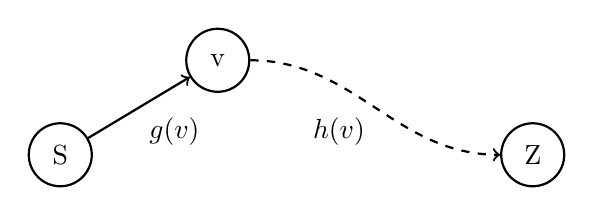
\begin{tikzpicture}
  [normalN/.style={circle,draw,minimum size=0.8cm},
   thick,auto,
   node distance=1.3cm]
   
  \node at (0,0)   [normalN] (start) {S};
  \node at (2,1.2) [normalN] (v)     {v};
  \node at (6,0)   [normalN] (ziel)  {Z};

  \draw [->] (start) to node [swap] {$g(v)$} (v);
  \draw [->,out=0,in=180,dashed] (v) to node [swap] {$h(v)$} (ziel);
\end{tikzpicture}
\caption{Prinzip des A*-Algorithmus}
\label{pic:AStern}
\end{figure}


Der A*-Algorithmus kann beispielsweise verwendet werden, um in einem Straßennetz die 
kürzeste Strecke zwischen zwei Städten zu finden. Die Funktion $g(v)$ gibt dabei die 
Strecke an, die tatsächlich gefahren werden muss, um eine Stadt zu erreichen. Als 
Abschätzung für $h(v)$ kann die Luftlinie zwischen zwei Städten benutzt werden, denn 
die direkte Verbindung ist immer kürzer als die tatsächliche Straßenlänge. 

\subsubsection{Anpassung an Graphabstand}
Zur Ermittlung des Graphabstands zweier Graphen $G_1$ und $G_2$ muss der 
Algorithmus leicht angepasst werden. Der Graph, in dem ein Pfad gesucht 
wird, ist der Suchbaum zur Ermittlung eines ECGMs. 
Startknoten ist die Wurzel des Baums. Zielknoten sind die Blätter. Der Wurzelknoten 
stellt ein "`leeres"' ECGM dar. Seine Unterknoten entsprechen nun allen möglichen 
Abbildungen des ersten Knotens aus $G_1$. Dazu gehört auch das Löschen des 
Knotens. \footnote{Aufgrund von Satz \ref{alleVausV1enthalten} (Abschnitt 
\ref{Vorueberlegungen}) ist es nicht nötig, das Löschen des Knotens zu betrachten, wenn 
$G_1$ der kleinere der beiden Graphen ist. Es werden dann sämtliche Knoten aus $G_1$ 
übernommen.} 

Aus dem Teil-ECGM, das durch einen Knoten $v$ des Suchbaums 
dargestellt wird, berechnen sich die bisherigen Kosten $g(v)$. 
In der in \cite{phdRiesen} vorgestellten Variante  ergeben sie 
sich aus den Kosten für das Hinzufügen und Entfernen von Kanten. Die noch anfallenden 
Kosten $h(v)$ berechnen sich aus dem Vergleich der Kanten, die noch nicht im aktuellen 
Teil-ECGM sind. Dabei wird ermittelt, wie viele Kanten mindestens entfernt bzw. hinzugefügt
werden müssen.

\subsubsection{Vergleich mit Branch-and-Bound}
Vergleicht man den A*- mit dem B\&B-Algorithmus, stellt man 
eine starke Ähnlichkeit fest. Beide Verfahren benutzen die 
gleiche Strategie: In einem zu durchsuchenden Graphen (bei 
B\&B immer ein Suchbaum) werden die bisher erreichten Knoten 
miteinander verglichen. An dem Knoten, dessen Summe aus den 
exakten und den erwarteten Kosten minimal ist, wird die 
Suche fortgesetzt. Der A*-Algorithmus ist dabei lediglich 
für eine Minimierung gedacht. Der B\&B-Algorithmus ist etwas 
allgemeiner formuliert. Es ist auch für eine Maximierung 
ausgelegt. Dies ist jedoch kein relevanter Unterschied. Beim 
B\&B-Algorithmus lassen sich Minimierung und Maximierung 
ineinander umwandeln, indem man die Kosten bzw. die Werte 
mit $-1$ multipliziert. 

Die in \cite{phdRiesen} beschriebene Methode zur Berechnung einer unteren Schranke 
für den Graphabstad zweier Graphen basiert auf dem gleichen Prinzip wie 
die Berechnung der Schranke in Abschnitt \ref{BBAlgo}. Es wird die Anzahl der 
verbliebenen Kanten im unbetrachteten Teil der Graphen miteinander verglichen. 
Das oben vorgestellte B\&B-Verfahren ermittelt dabei die Anzahl der gemeinsamen 
Kanten. Die in \cite{phdRiesen} vorgestellte Variante zur Berechnung einer unteren 
Schranke (der noch anfallenden Kosten $h(v)$) berechnet die Zahl der zu löschenden 
Kanten. Addiert man beides, erhält man somit die Gesamtzahl der Kanten. Da diese 
für ein Graphenpaar konstant ist, sind auch beide Schranken äquivalent zueinander. 
Aus diesem Grund wird in Kapitel \ref{chp:AlgoTest} lediglich der B\&B-Algorithmus
betrachtet.

\subsection{Bipartite Heuristik}
Eine mögliche Variante, um den Graphabstand zweier Graphen abzuschätzen, ist ein 
Matching auf einem bipatiten Graphen.


\subsubsection{Grundlagen}
Ein bipartiter Graph zeichnet sich dadurch aus, dass sich dessen Knotenmenge 
in zwei Teilmengen unterteilen lässt, wobei Kanten immer jeweils einen Knoten 
der einen mit einem Knoten der anderen Teilmenge verbinden. Zwischen den Knoten 
innerhalb einer Teilmenge gibt es keine Kanten.

\begin{mydef}[bipartiter Graph]
Ein gewichteter bipartiter Graph $G$ ist ein 3-Tupel $G=(V,E,\omega)$. Dabei sind:
\begin{itemize}
	\item $V=V_1 \cup V_2$ mit $V_1 \cap V_2=\emptyset$ eine endliche Menge an Knoten,
	\item $E \subseteq V_1 \times V_2$ die Menge der Kanten und
	\item $\omega:E \rightarrow \mathbb{Q}$ die Gewichtsfunktion der Kanten.
\end{itemize}
$G$ ist \emph{voll} genau dann, wenn $E=V_1\times V_2$.
\end{mydef}

Bei einem Matching in einem Graphen werden Knoten einander zugeordnet. Dabei müssen 
die Knoten über eine Kante miteinander verbunden sein. Diese Zuordnung ist eindeutig. 
Es wird also jedem Knoten nur maximal ein anderer Knoten zugeordnet.

\begin{mydef}[Matching]
Ein Matching in einem gewichtetem bipartiten Graphen $G=(V_1 \cup V_2,E,\omega)$ ist eine bijektive
Abbildung $\mu:\hat{V_1} \rightarrow \hat{V_2}$ mit $\hat{V_1} \subseteq V_1$ und $\hat{V_2}
 \subseteq V_2$. Dabei gilt: $v \in \hat{V_1} \Rightarrow (v,\mu(v)) \in E$.
\end{mydef}

Das Gewicht $w$ eines Matchings ist dann: 
\[ w=\sum_{v \in \hat{V_1}} \omega((v,\mu(v)))  \]

\subsubsection{Arbeitsweise}
Idee der Heuristik ist, dass man ein ECGM auch als Matching in einem bipartiten Graphen
interpretieren kann. Gegeben seien die Graphen $G_1=(V_1,E_1)$ und $G_2=(V_2,E_2)$
mit $n=|V_1|$ und $m=|V_2|$. Daraus lässt sich nun
ein voller bipartiter Graph $M=(V_M,E_M,\omega)$ wie folgt erstellen:
\begin{itemize}
	\item $V_M=(V_1 \cup \{\varepsilon_{1_1},\ \ldots\ , \varepsilon_{1_m}\}) \cup
	           (V_2 \cup \{\varepsilon_{2_1},\ \ldots\ , \varepsilon_{2_n}\})$
	\item $E_M=(V_1 \cup \{\varepsilon_{1_1},\ \ldots\ , \varepsilon_{1_m}\}) \times
	           (V_2 \cup \{\varepsilon_{2_1},\ \ldots\ , \varepsilon_{2_n}\})$
\end{itemize}
Der eine Teil der Knoten in $M$ ergibt sich aus den Knoten in $G_1$ sowie 
je einem $\varepsilon$-Knoten für jeden Knoten in $G_2$. Der zweite Teil 
bildet sich analog: es werden die Knoten aus $G_2$ genommen, sowie je ein 
$\varepsilon$-Knoten für jeden Knoten in $G_1$.

Die $\varepsilon$-Knoten dienen dazu, um das Hinzufügen oder Entfernen von Knoten 
ebenfalls als Matching zu ermöglichen. Wird ein Knoten hinzugefügt, so wird ihm ein 
$\varepsilon$-Knoten zugeodnet: $\varepsilon_{1_i} \mapsto v_i$. Beim Löschen 
ist es andersrum: $v_i \mapsto \varepsilon_{2_i}$.

 Ein ECGM ist nun äquvalent zu einem Matching in $M$. 
Die Kosten $c_{u v}$, die mindestens entstehen, wenn zwei Knoten $u$ und $v$ einander 
zugewiesen werden, ergeben dann die Kantengewichte von $M$. Zur Berechnung der Kosten 
werden die Kanten von $G_1$ und $G_2$ 
mit einbezogen. Hat beispielsweise ein Knoten drei Kanten und wird auf einen Knoten mit 
fünf Kanten abgebildet, so müssen mindestens zwei Kanten entfernt oder hinzugefügt werden. 
Die Kosten können als Kosten-Matrix $C$ dargestellt werden. 

\[
C=\left [
\begin{array}{ccc|ccc}
c_{11} & \cdots & c_{1 m} & c_{1\varepsilon} &        & \infty \\
\vdots & \ddots & \vdots &                  & \ddots & \\
c_{n 1} & \cdots & c_{n m} & \infty           &        & c_{n\varepsilon} \\

\cline{1-6}

c_{\varepsilon 1} &        & \infty            & &   & \\
                  & \ddots &                   & & 0 & \\
\infty            &        & c_{\varepsilon m} & &   &

\end{array} \right ]
\]

Die Matrix ist in vier Bereiche unterteilt. Oben links befinden sich die Kosten, 
die beim Zuweisen eines Knoten aus $G_1$ zu einem Knoten aus $G_2$ auftreten. Oben 
rechts und unten links sind die Kosten für das Hinzufügen oder Löschen von Knoten. 
Die Kosten stehen jedoch nur in den Diagonalen. Alle anderen Werte sind unendlich. 
Im unteren rechten Teil sind alle Werte null. Sie stellen den Fall dar, dass zwei 
$\varepsilon$-Knoten einander zugewiesen werden.

Um nun ein ECGM zu finden, das möglichst geringe Kosten hat, wird das Matching gesucht, 
dessen Gewicht minimal ist. Dieses lässt sich durch ein Verfahren ermitteln, welches als 
Ungarische Methode\footnote{Es ist auch unter Munkres Algorithmus oder 
Kuhn-Munkres-Algorithmus bekannt.} bekannt ist. Die Methode findet ein minimales Matching 
in $\mO(n^3)$ \cite{Munkres1957}. 

\subsubsection{Matching als untere Schranke}
In \cite{RiesenSpeedingup} wird die Heuristik als mögliche Abschätzung für die 
mindestens noch entstehenden Kosten ($h$-Funktion) und somit als untere 
Schranke zur Berechnung des Graphabstands mittels eines A*-""Algorithmus vorgeschlagen. 
Die Argumentation dabei ist, dass 
die Kantengewichte des bipartiten Graphen jeweils die minimalen Kosten 
für das Abbilden der Knoten aufeinander darstellen. Somit sei das minimale 
Gesamtgewicht eines Matchings auch die minimalen Kosten für den gesamten 
Graph. Bewiesen wird diese Behauptung nicht. 
Bei einer genauen Betrachtung stellt sich diese Aussage hingegen als inkorrekt heraus. 
 Es kann passieren, dass Kosten für Kanten doppelt 
berechnet werden. Dies liegt daran, dass die Kosten an beiden Knoten der Kante 
erhoben werden.

%\begin{figure}[htb]
%\centering
%\hspace*{\fill}
%\subfloat[\label{pic:bspBipMatching1}]{\includegraphics[width=0.3\linewidth,
%keepaspectratio]{bilder/bspBipMatching1}}
%\hspace*{\fill}
%\subfloat[\label{pic:bspBipMatching2}]{\includegraphics[width=0.3\linewidth,
%keepaspectratio]{bilder/bspBipMatching2}}
%\hspace*{\fill}
%\caption{Graphen, die sich durch genau eine Kante unterscheiden}
%\label{pic:BspBipMatching}
%\end{figure}

\begin{figure}[htb]
\centering
\hspace*{\fill}
\subfloat[\label{pic:bspBipMatching1}]{\begin{tikzpicture}
  [normalN/.style={circle,draw,minimum size=0.8cm,thick},
   node distance=1.3cm]

  \node[normalN] (a) {1};
    
  \node[normalN] (b) [right=of a] {2}
    edge [thick] (a);
    
  \node[normalN] (c) [below=of b] {3}
    edge [thick] (b)
    edge [thick] (a);
    
  \node[normalN] (d) [left=of c] {4}
    edge [thick] (a)
    edge [thick] (c);
  
\end{tikzpicture}}
\hspace*{\fill}
\subfloat[\label{pic:bspBipMatching2}]{\begin{tikzpicture}
  [normalN/.style={circle,draw,minimum size=0.8cm,thick},
   node distance=1.3cm]

  \node[normalN] (a) {a};
    
  \node[normalN] (b) [right=of a] {b}
    edge [thick] (a);
    
  \node[normalN] (c) [below=of b] {c}
    edge [thick] (b);
    
  \node[normalN] (d) [left=of c] {d}
    edge [thick] (a)
    edge [thick] (c);
  
\end{tikzpicture}}
\hspace*{\fill}
\caption{Graphen, die sich durch genau eine Kante unterscheiden}
\label{pic:BspBipMatching}
\end{figure}

Die in Abbildung \ref{pic:BspBipMatching} dargestellen Graphen sind bis auf die Kante 
in der Mitte gleich. Der Graphabstand entspricht somit lediglich dem Hinzufügen oder Entfernen 
der Kante. Die Kosten werden allerding zweimal in die Kostenmatrix übernommen und 
auch zweimal in das Gesamtgewicht des Matchings eingerechnet. 

Setzt man die Kosten für das Einfügen und Löschen von Knoten und Kanten jeweils auf $1$,
so ergibt sich folgende Kostenmatrix $C$:

\[
C=\left [
\begin{array}{cccc|cccc}
    1 & 1 & 1 & 1 & 3 &   &   & \infty \\
    0 & 0 & 0 & 0 &  & 2 &   &  \\
    1 & 1 & 1 & 1 &   &   & 3 &  \\
    0 & 0 & 0 & 0 &  \infty &   &   & 2 \\
 \cline{1-8}
         2 &   &   & \infty & \multicolumn{4}{c}{\multirow{4}{*}{0}}\\
           & 2 &   &  \\
           &   & 2 &  \\
    \infty &   &   & 2 \\

\end{array} \right ] 
\]

Ein minimales Matching ergibt sich nun aus folgenden Abbildungen:
%\begin{align*}
\[
\begin{array}{ccc}
	1 & \longmapsto & a \\
  2 & \longmapsto & b \\
  3 & \longmapsto & c \\
  4 & \longmapsto & d \\
	\varepsilon_{1,\ldots,4} & \longmapsto & \varepsilon_{a,\ldots,d}
\end{array}	
\]%\end{align*}

%\[
%\begin{array}{ccc}
%	1 & \longmapsto & a \\
%	  & \vdots & \\
%  4 & \longmapsto & d \\
%	\varepsilon_1 & \longmapsto & \varepsilon_a \\
%	  & \vdots & \\
%	\varepsilon_4 & \longmapsto & \varepsilon_d
%\end{array}	
%\]%\end{align*}

Die in $C$ eingetragenen Kosten für $1 \mapsto a$ und  $3 \mapsto c$ 
sind jeweils $1$. Das minimale Gesamtgewicht ist somit $2$. Der
Graphabstand ist jedoch nur $1$. Das Gewicht des Matchings liegt somit
über den eigentlichen Kosten und kann keine untere Schranke sein.

\section{Zusammenfassung}
Es wurden nun  fünf Algorithmen vorgestellt, um den Graphabstand 
zweier Graphen zu ermitteln. Diese verfolgen dabei unterschiedliche 
Ansätze. Zwei dieser Algorithmen erwiesen sich als 
so ähnlich, dass nur einer von ihnen weiter betrachtet wird. 
Zwei weitere Algorithmen sind lediglich inexakte Verfahren, bei denen nicht sicher ist, 
dass die ermittelte Lösung auch die beste ist.

Das nächste Kapitel vergleich nun diese Algorithmen und versucht Aussagen über 
deren Geschwindigkeit und (bei den inexakten Verfahren) über die Qualität der 
Lösungen zu treffen.